
\chapter{Analisi dei requisiti}
\label{cap:analisi-requisiti}

\intro{In questo capitolo viene presentata l'analisi dei requisiti effettuata
    durante lo stage, dove si mostrano le funzionalità e i requisiti individuati, al
    fine di fornire una visione più chiara del sistema.}\\

\section{Descrizione dell'applicazione}
Il progetto consiste nel creare un servizio per la
conversione di vari formati immagine. Il prodotto vuole essere una
sperimentazione interna per la sostituzione di un servizio interno che svolge
già lo stesso compito, utilizzando delle tecnologie \emph{cloud-native} e
\emph{serverless}, al fine di semplificare il flusso della conversione e di
fornire uno strumento più mantenibile e scalabile rispetto al precedente.\\


\section{Casi d'uso}

Per lo studio dei casi di utilizzo del prodotto sono stati creati dei diagrammi.
I diagrammi dei casi d'uso (in inglese \emph{Use Case Diagram}) sono diagrammi
di tipo \emph{UML} dedicati
alla descrizione delle funzioni o servizi offerti da un sistema, così come sono
percepiti e utilizzati dagli attori che interagiscono col sistema stesso.
Essendo il progetto finalizzato alla creazione di un servizio che richiede
attualmente solo un intervento minimo da parte dell'utente, i diagrammi risultano semplici ed in numero ridotto.

\subsection{Descrizione del sistema}
Di seguito viene rappresentato un diagramma riassuntivo che mostra i casi d'uso
individuati e le relazioni tra essi.

\begin{usecase}{1}{Recupero dell'immagine}
    \begin{figure}[H]
        \centering
        
\includegraphics[width=0.8\textwidth]{images/uc1.png}
        \caption{UC$1$ - Recupero dell'immagine}
    \end{figure}
    \label{fig:uc1}
    \usecaseactors{\emph{Lambda}, \emph{bucket S3} di input delle immagini}
    \usecasepre{La funzione \emph{Lambda} è pronta per l'esecuzione e l'immagine da convertire è caricata nel \emph{bucket S3} di \emph{input}}
    \usecasedesc{All'interno della \emph{Lambda} viene effettuata una richiesta con il nome dell'immagine al \emph{bucket S3} e viene effettuato il download nella memoria interna della \emph{Lambda}}
    \usecasepost{La \emph{Lambda} ha l'immagine salvata in memoria, al fine di procedere con la conversione}
    \label{uc:recupero-immagine}
\end{usecase}

\begin{usecase}{2}{Recupero configurazione della conversione}
    \begin{figure}[H]
        \centering
        
\includegraphics[width=0.8\textwidth]{images/uc2.png}
        \caption{UC$2$ - Recupero configurazione della conversione}
    \end{figure}
    \usecaseactors{\emph{Lambda}, tabella \emph{DynamoDB}}
    \usecasepre{La funzione \emph{Lambda} è pronta per l'esecuzione e la configurazione della conversione è salvata nella tabella \emph{DynamoDB}}
    \usecasedesc{All'interno della \emph{Lambda} viene effettuata una richiesta con l'\emph{ID} del cliente che ha richiesto la conversione alla tabella \emph{DynamoDB} contenente le configurazioni, suddivise per cliente, e vengono impostate le specifiche desiderate}
    \usecasepost{La \emph{Lambda} ha la configurazione della conversione salvata in memoria, al fine di procedere con la conversione}
    \label{uc:recupero-configurazione}

\end{usecase}

\begin{usecase}{3}{Esecuzione della conversione}
    \begin{figure}[H]
        \centering
        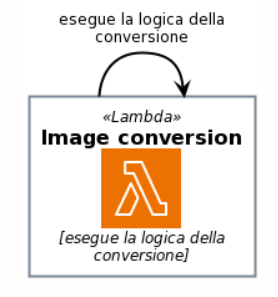
\includegraphics[width=0.3\textwidth]{images/uc3.png}
        \caption{UC$3$ - Esecuzione della conversione}
    \end{figure}
    \usecaseactors{\emph{Lambda}}
    \usecasepre{La funzione \emph{Lambda} è pronta per l'esecuzione, l'immagine da convertire e la configurazione sono state salvate nella memoria temporanea della \emph{Lambda}}
    \usecasedesc{La funzione \emph{Lambda} effettua la conversione dell'immagine
        secondo la configurazione desiderata. Se la conversione va a buon fine,
        l'immagine convertita viene salvata nella memoria temporanea della \emph{Lambda},
        contraddistinta da un nome composto da un \emph{ID} univoco, il
        nome dell'immagine e il nome della configurazione utilizzata}
    \usecasepost{La \emph{Lambda} ha l'immagine convertita nella sua memoria temporanea e vengono salvate le caratteristiche della conversione in una variabile}
    \label{uc:esecuzione-conversione}

\end{usecase}
\begin{usecase}
    {4}{Salvataggio dell'immagine convertita}
    \begin{figure}[H]
        \centering
        
\includegraphics[width=0.8\textwidth]{images/uc4.png}
        \caption{UC$4$ - Salvataggio dell'immagine convertita}
    \end{figure}
    \usecaseactors{\emph{Lambda}, \emph{bucket S3} di output delle immagini}
    \usecasepre{La funzione \emph{Lambda} è pronta per iniziare l'\emph{upload} dell'immagine e l'immagine convertita è salvata nella memoria temporanea della \emph{Lambda}}
    \usecasedesc{La funzione \emph{Lambda} effettua il caricamento dell'immagine convertita nel \emph{bucket S3} di output delle immagini, inserendola in una sottocartella contraddistinta dal nome del cliente che ha richiesto la conversione}
    \usecasepost{L'immagine convertita è salvata nel \emph{bucket S3} di \emph{output} delle immagini nella cartella del cliente che ha richiesto la conversione}
    \label{uc:salvataggio-immagine}
\end{usecase}
\begin{usecase}{5}{Salvataggio caratteristiche della conversione}
    \begin{figure}[H]
        \centering
        
\includegraphics[width=0.8\textwidth]{images/uc5.png}
        \caption{UC$5$ - Salvataggio caratteristiche della conversione}
    \end{figure}
    \usecaseactors{\emph{Lambda}, tabella \emph{DynamoDB} contenente tutte le conversioni effettuate}
    \usecasepre{La funzione \emph{Lambda} è pronta per scrivere le caratteristiche
        della conversione in una tabella di \emph{DynamoDB} dedicata}
    \usecasedesc{La funzione Lambda effettua il salvataggio delle caratteristiche della conversione nella tabella \emph{DynamoDB}, contraddistinta da un \emph{ID} univoco, il nome dell'immagine e il nome della configurazione utilizzata}
    \usecasepost{Le caratteristiche della conversione sono salvate nella tabella \emph{DynamoDB}}
    \label{uc:salvataggio-caratteristiche}
\end{usecase}

\section{Tracciamento dei requisiti}

Sono stati individuati diversi tipi di requisiti e si è quindi fatto utilizzo di
un codice identificativo per distinguerli, rappresentato di seguito:
\begin{itemize}
    \item \textbf{Requisiti funzionali:} descrivono le funzioni che il sistema
          deve offrire. Delineano le azioni che il sistema deve eseguire, le
          risposte attese da determinati input e le dinamiche generali del sistema;
    \item \textbf{Requisiti qualitativi:} descrivono le caratteristiche che il
          sistema deve possedere, legati alla qualità e alle prestazioni del sistema;
    \item \textbf{Requisiti di vincolo:} descrivono i parametri che il sistema
          deve rispettare durante lo sviluppo e l'implementazione.
\end{itemize}
Viene inoltre fatta una classificazione dei requisiti in base alla loro
priorità.

\subsection{Notazione}
Ciascun requisito è identificato da un codice univoco, che aderisce alla
seguente notazione:
\begin{center}
    \textbf{R[Priorità][Tipo]-[Codice]}
\end{center}
dove:
\begin{itemize}
    \item \textbf{Priorità:} può assumere i seguenti valori:
          \begin{itemize}
              \item \textbf{O:} requisito obbligatorio;
              \item \textbf{D:} requisito desiderabile;
              \item \textbf{Z:} requisito opzionale.
          \end{itemize}
          \newpage
    \item \textbf{Tipo:} può assumere i seguenti valori:
          \begin{itemize}
              \item \textbf{F:} requisito funzionale;
              \item \textbf{Q:} requisito qualitativo;
              \item \textbf{V:} requisito di vincolo.
          \end{itemize}
    \item \textbf{Codice:} è un codice identificativo univoco del requisito.
\end{itemize}

Nelle tabelle \ref{tab:requisiti-funzionali}, \ref{tab:requisiti-qualitativi} e
\ref{tab:requisiti-vincolo} sono riassunti i requisiti e il loro tracciamento
con i casi d'uso delineati in fase di analisi.
\newpage

\subsection{Requisiti funzionali}
\begin{table}[H]
    \caption{Tabella del tracciamento dei requisti funzionali}
    \label{tab:requisiti-funzionali}
    \begin{tabularx}{\textwidth}{|c|X|c|}
        \hline
        \textbf{Requisito} & \textbf{Descrizione}                                            & \textbf{Use Case} \\
        \hline
        %Add requirements based on use case
        ROF-1              & Recuperare le immagini da convertire da un bucket S3
                           & UC1
        \\
        \hline
        ROF-2              & Utilizzare dei parametri in formato JSON per la
        configurazione di una conversione
                           & UC2
        \\
        \hline
        ROF-3              & Permettere una conversione da formato JPG al
        formato JPG        & UC3
        \\
        \hline
        ROF-4              & Permettere una conversione da formato WEBP al formato JPG       & UC3
        \\
        \hline
        ROF-5              & Permettere una conversione da formato PNG al formato PNG        & UC3
        \\
        \hline
        ROF-6              & Permettere una conversione da formato SVG al formato PNG        & UC3
        \\
        \hline
        ROF-7              & Permettere una conversione da formato TIFF al formato PNG       & UC3
        \\
        \hline
        ROF-8              & Permettere una conversione da formato GIF al formato PNG        & UC3
        \\
        \hline
        ROF-9              & Permettere una conversione da formato BMP al formato PNG        & UC3
        \\
        \hline
        ROF-10             & Permettere una conversione da formato ICO al formato PNG        & UC3
        \\
        \hline
        ROF-11             & Permettere una conversione da formato PSD al formato PNG        & UC3
        \\
        \hline
        ROF-12             & Permettere una conversione da formato AI al formato PNG         & UC3
        \\
        \hline
        ROF-13             & Permettere una conversione da formato EPS al formato PNG        & UC3
        \\
        \hline
        ROF-14             & Permettere una conversione da formato PS al formato PNG         & UC3
        \\
        \hline
        ROF-15             & Permettere una conversione da formato Postscript al formato PNG
                           & UC2
        \\
        \hline
        ROF-16             & Permettere una conversione da formato ARW al formato PNG        & UC3
        \\
        \hline
        ROF-17             & Permettere una conversione da formato CR2 al formato PNG        & UC3
        \\
        \hline
        ROF-18             & Permettere una conversione da formato DNG al formato PNG        & UC3
        \\
        \hline
    \end{tabularx}
\end{table}%
\newpage
\begin{table}[H]
    \begin{tabularx}{\textwidth}{|c|X|c|}
        \hline

                                        & \centering \textbf{Continuazione della tabella
        \ref{tab:requisiti-funzionali}} &
        \\
        \hline
        \textbf{Requisito}              & \textbf{Descrizione}                                               & \textbf{Use Case} \\
        \hline
        ROF-19                          & Permettere una conversione da formato NEF al formato PNG           & UC3
        \\
        \hline
        ROF-20                          & Permettere una conversione da formato ORF al formato PNG           & UC3
        \\
        \hline
        ROF-21                          & Permettere una conversione da formato RAF al formato PNG           & UC3
        \\
        \hline
        ROF-22                          & Impedire l'upscaling di una immagine
                                        & UC3                                                                                    \\
        \hline
        ROF-23                          & Convertire il profilo colore dell'immagine
                                        & UC3                                                                                    \\
        \hline
        ROF-24                          & Mantenere la trasparenza dell'immagine, se prevista
                                        & UC3                                                                                    \\
        \hline
        ROF-25                          & Effettuare, se possibile, il downscale
        dell'immagine secondo la risoluzione desiderata
                                        & UC3                                                                                    \\
        \hline
        ROF-26                          & Permettere la conversione di più immagini in una
        singola esecuzione
                                        & UC3
        \\
        \hline
        ROF-27                          & Permettere la conversione di più immagini ad una
        diversa risoluzione durante una singola esecuzione
                                        & UC3
        \\
        \hline
        ROF-28                          & Effettuare l'estrazione del formato originale dell'immagine
                                        & UC3
        \\
        \hline

        ROF-29                          & Effettuare l'estrazione della risoluzione originale dell'immagine
                                        & UC3
        \\
        \hline
        ROF-30                          & Effettuare l'estrazione del profilo colore originale dell'immagine
                                        & UC3
        \\
        \hline
        ROF-31                          & Effettuare l'estrazione della dimensione in byte
        dell'immagine originale
                                        & UC3
        \\
        \hline
        ROF-32                          & Individuare la presenza del canale alfa per la
        trasparenza dell'immagine
                                        & UC3
        \\
        \hline
        ROF-33                          & Effettuare il salvataggio dell'immagine convertita
        in un percorso specifico
                                        & UC4
        \\
        \hline

        ROF-34                          & Salvare le informazioni legate alla conversione in
        campi strutturati               & UC5
        \\
        \hline
    \end{tabularx}
\end{table}
\subsection{Requisiti qualitativi}
\begin{table}[H]
    \caption{Tabella del tracciamento dei requisiti qualitativi}
    \label{tab:requisiti-qualitativi}
    \begin{tabularx}{\textwidth}{|c|X|c|}
        \hline
        \textbf{Requisito}                  & \textbf{Descrizione}                    & \textbf{Use Case} \\
        \hline
        ROQ-1                               & Il progetto deve essere accompagnato da
        documentazione tecnica e funzionale & Interno                                                     \\
        \hline
        ROQ-2                               & Il codice deve essere accompagnato
        da test di unità e di sistema       & Interno
        \\
        \hline
        ROQ-3                               & Scrivere dei log per ogni
        operazione effettuata, inserendo sempre l'ID della conversione
                                            & Interno
        \\
        \hline
    \end{tabularx}
\end{table}

\subsection{Requisiti di vincolo}
\begin{table}[H]
    \caption{Tabella del tracciamento dei requisiti di vincolo}
    \label{tab:requisiti-vincolo}
    \begin{tabularx}{\textwidth}{|c|X|c|}
        \hline
        \textbf{Requisito}                                               & \textbf{Descrizione}                                & \textbf{Use Case} \\
        \hline
        ROV-1                                                            & Il servizio deve essere implementato utilizzando il
        linguaggio di programmazione \emph{Go}                           & UC1                                                                     \\
        \hline
        ROV-2                                                            & Il servizio deve utilizzare l'istanza
        \emph{Lambda} di \emph{AWS} per
        l'esecuzione del codice                                          & UC2                                                                     \\
        \hline
        ROV-3                                                            & Il servizio deve utilizzare il sistema di
        persistenza \emph{DynamoDB} di \emph{AWS} per i dati strutturati & UC1
        \\
        \hline
        ROV-4                                                            & Il servizio deve utilizzare il sistema di
        persistenza \emph{S3} di \emph{AWS} per i dati non strutturati   & UC1
        \\
        \hline
        RDV-5                                                            & Il
        servizio deve integrare i log con il sistema di monitoraggio
        \emph{CloudWatch} di \emph{AWS}                                  & UC3
        \\
        \hline
        RZV-6                                                            & Il
        servizio deve esporre delle \emph{API REST} per il recupero dei
        \emph{job} di conversione da parte del team di \emph{frontend}   & UC3                                                                     \\
        \hline
    \end{tabularx}
\end{table}%
